%Schriftgröße, Dokumentformat, Dokumenttyp
\documentclass[11pt,a4paper]{article}
%Einstellungen der Seitenränder
\usepackage[left=3cm,right=4cm,top=2cm,bottom=2cm,includeheadfoot]{geometry}
%neue Rechtschreibung und Formelsatz
\usepackage[utf8]{inputenc}
\usepackage[english]{babel}
\usepackage[T1]{fontenc}
\usepackage{textcomp}
\usepackage{amsmath,amssymb,amsthm}
%Graphiken
\usepackage{graphicx}
\usepackage{float}
%Zeilenabstand
\usepackage{setspace}\onehalfspacing
%Aufzählungen
\usepackage{paralist}
%Abkürzungen
\usepackage{acronym}
%Tabelle
\usepackage{multirow}
%Kopf- und Fußzeile
\usepackage{fancyhdr}
%Fußnotenkram
\usepackage{footnote}
\usepackage{hyperref}
\usepackage[hang]{footmisc}
\usepackage{graphics}
\usepackage{glossaries}
\setlength{\footnotesep}{0.25 cm}

% HINZUGEFÜGT VON ADRIAN
% MAKE subsubsubsection possible
\usepackage{titlesec}
\usepackage[nottoc]{tocbibind}
\usepackage{cleveref}
\usepackage{acronym}
\usepackage[toc,page]{appendix}
%\usepackage{subfig}
\graphicspath{{./img/}}
\usepackage{caption}
\usepackage[yyyymmdd]{datetime}
\usepackage{subcaption}
\usepackage{bbm}
%\usepackage[demo]{graphicx}


% ACRONYMS 
\newacro{MSGARCH}{Markov-Switching GARCH}
\newacro{GARCH}{General Autoregressive Conditional Heteroskedasticity}
\newacro{ARCH}{Autoregressive Conditional Heteroskedasticity}
\newacro{ARMA}{AutoRegressive Moving Average}
\newacro{SGED}{Skewed Generlized Error Distribution}
\newacro{GED}{Generalized Error Distribution}
\newacro{MSE}{mean-square error}
\newacro{MAE}{mean-absolute error}
\newacro{RMSE}{root-mean-square error}
\newacro{MSM}{Markov-Switching Model}
\newacro{HMM}{Hidden Markov Model}
\newacro{CRPS}{Continuous Ranked Probability Score}
\newacro{cdf}{cumulative density function}
\newacro{MSM}{markov-switching models}

\setcounter{secnumdepth}{4}

\titleformat{\paragraph}
{\normalfont\normalsize\bfseries}{\theparagraph}{1em}{}
\titlespacing*{\paragraph}
{0pt}{3.25ex plus 1ex minus .2ex}{1.5ex plus .2ex}
%


\begin{document}
% Keine Seitenzahlen im Vorspann
\pagestyle{empty}
	
%%%%%%%%%%%%%%%%%%%%%%% Titelblatt der Arbeit %%%%%%%%%%%%%%%%%%%%%%%
\begin{titlepage}				
	\begin{center}
Professorship for XXX\\
Institute of XXX\\
Faculty of Business, Economics and Social Sciences\\
Kiel University \\
		\vspace{5cm}
		
		\LARGE{ \bf{Density Forecasts of the S\&P using Markov-Switching Models}}
		\vspace{2cm}
		
		\large{\bf{Seminar paper}}\\
		Submission Date: XX.XX.XXXX
		\vspace{1.5cm}

\begin{flushleft}
\vfill
	Author: Adrian Beer
	Subject:\\
	Semester:3
	Module: Seminar in Econometrics
	Stu-Email-Adress:\\
	Matriculation number:\\
	\vspace{1cm}
	First Assessor:\\
	Second Assessor:
\end{flushleft}	
		
				
	\end{center}

\end{titlepage}


%%%%%%%%%%%%%%%%%%%%%%% Inhaltsverzeichnis %%%%%%%%%%%%%%%%%%%%%%%


\newpage
	\tableofcontents
	\newpage


% Kopf- und Fußzeile definieren 
\pagestyle{fancy}					
\fancyhf{}								
%Kopfzeile rechts bzw. außen			
\fancyhead[R]{}							 
%Linie oben								 
\renewcommand{\headrulewidth}{0pt}	 
%Fußzeile mittig					 
\fancyfoot[R]{\thepage}				 
%Linie unten										
\renewcommand{\footrulewidth}{0pt}	 
%Seitenzahlen ab hier						 
\pagenumbering {Roman} 
\setcounter{page}{1}



%%%%%%%%%%%%%%%%%%%%%%%%%%%%% List of Figures %%%%%%%%%%%%%%%%%%%%%%%%%%%%%%%%%
\addcontentsline{toc}{section}{Figure directory}
\listoffigures


\newpage
%%%%%%%%%%%%%%%%%%%%%%%%%%%%% List of Tables %%%%%%%%%%%%%%%%%%%%%%%%%%%%%%%%%
\addcontentsline{toc}{section}{Table directory}
\listoftables
\newpage

%%%%%%%%%%%%%%%%%%%%%%%%%%%%% List of Symbols %%%%%%%%%%%%%%%%%%%%%%%%%%%%%%%
\section*{List of Symbols} 
\addcontentsline{toc}{section}{Symbol directory}
\noindent Include a symbol directory if you use more than three uncommon abbreviations.
	\begin{tabular}{l l}
		\textbf{} & \\
		$\sigma$ & standard deviation\\
		$\Psi$ & set of parameter values \\
		$h$ conditional variance
	\end{tabular}\\ \vspace{1cm}


\newpage


% Kopf- und Fußzeile definieren %%
\pagestyle{fancy}						
\fancyhf{}								
%Kopfzeile rechts bzw. außen			
\fancyhead[R]{}							 
%Linie oben								 
\renewcommand{\headrulewidth}{0pt}	 
%Fußzeile mittig					 
\fancyfoot[R]{\thepage}				 
%Linie unten										
\renewcommand{\footrulewidth}{0pt}	 
%Seitenzahlen ab hier						 
\pagenumbering {arabic}
\onehalfspacing	
\section{Introduction}
Markov chain processes can be useful for identifying regimes in the past as well as estimating the current regime. %% why is this important
If the \ac{MSM} describes the data generating process well, it can also be used to simulate synthetic time series and potential future paths. %% why is this important

\ac{MSM}s have been a popular approach in modelling non-linear time series dynamics.

\ac{GARCH} models are widely used in order to describe the behaviour of financial time series.
In this work we want to assess in a case study, if a markov-switching will improve the forecasts of a stand-alone GARCH model.


\section{Background}
\subsection{Markov-Switching Models}
The general model consists of two stochastic processes $X$ and $Y$. The process $Y$ is observed, e.g. the stock price of a company, and it's conditional distribution depends on the unobserved Markov chain process $X$. According to \cite{an_identifiability_2013}, when the distribution of $y_t$ depends only on $x_t$ it is called a \ac{HMM}, and if it additionally depends  on the lagged values $y_{t-1}, ... y_{t-l}$ we call it a \ac{MSM}.

There are two main ways to learn the parameters of a HMM model: Expectation-Maximization Algorithms (EM) such as Baum-Welch. And Markov Chain Monte Carlo methods (MCMC) such as the Metropolis-Hastings or Gibbs Sampling algorithm.

The EM Algorithm makes use of the forward-backward algorithm.

Given a HMM model we can deduce estimates of the hidden state via the Viterbi algorithm.

Our goal is to maximize the incomplete data log-likelihood 
$$\log f(y \mid X ; \theta)=\log \sum_{s_{1}=1}^{2} \sum_{s_{2}=1}^{2} \ldots \sum_{s_{T}=1}^{2} f(y, s \mid X ; \theta)$$ which is not feasible to compute (complexity).


$$ \mathcal{L}\left(\Psi \mid \mathcal{I}_T\right) \equiv \prod_{t=1}^T f\left(y_t \mid \Psi, \mathcal{I}_{t-1}\right) $$ 

\subsubsection{Exogeneous Variables}
\paragraph{Time-varying transition probabilities}
Most HMMs are trained based on an purely endogeneous variables. One way to introduce exogeneous variables X into the HMM is by using them to estimate time-varying transition probabilities. This concept has been introduced by Diebold et al. \cite{diebold_regime_1993} together with closed form solutions for Gaussian state probability distributions. Since the complexity of calculating the expected likelihood for the EM algorithm in this setting is squared in the number of observations, maximizing it numerically with respect to the parameters is computationally not feasible. Since no closed form solutions to the maximization step for any fat-tailed distributions are available in this setting, this is currently not suited to model financial market data.

\paragraph{State-space model/ DFM-MSs}
Another way to integrate outside information is to use state space models. In this setting the state is represented by one or more so called dynamic factors whose behaviour is specified in the state equation and its relation to the variable of interest in the output equation. The usefulness of this approach depends on two factors: the dynamic factor has to be somewhat predictable and 
needs to explain the output variable reasonably well. The state space model can be learned using the Kalman filters in Gaussian settings or using MCMC methods otherwise.

\subsection{Financial Markets}

\subsubsection{Stylized Facts about returns and volatility}
Volatility is standard deviation of the log returns.
Fat-tailed. Power-law. Daily vs Monthly frequencies. 

\subsubsection{Distributions}
Many different distributions have been suggested for modeling asset returns and volatility, among them the log-normal, students-t and the \ac{GED} and stable tempered distributions. 
In this paper we will consider  \ac{GED}, given the difficulty of implementing algorithms using more advanced distributions such as the stable tempered distribution. 

\paragraph{Generalized Error Distribution}
\begin{equation} \label{eq:ged}
f_{\mathrm{GED}}(\eta ; \nu) \equiv \frac{\nu e^{-\frac{1}{2}|\eta / \lambda|^\nu}}{\lambda 2^{(1+1 / \nu)} \Gamma(1 / \nu)}, \quad \lambda \equiv\left(\frac{\Gamma(1 / \nu)}{4^{1 / \nu} \Gamma(3 / \nu)}\right)^{1 / 2}
\end{equation}
where $\nu$ is the shape parameter and $\lambda$ the scale parameter the density function.

\paragraph{Skewness}
Since the densities of financial stochastic processes are usually skewed, a method of introducing this property to the symmetric density \cref{eq:ged} is required. Given a standardized, symmetric unimodal density, Trottier and Ardia suggest the following transformation, which doesn't change neither the mean nor the variance (see \cite{trottier_moments_2015}). The degree of skewness is parametrized by $0<\xi<\infty$:
\begin{equation} \label{eq:skewness}
	f_{\xi}(z) \equiv \frac{2 \sigma_{\xi}}{\xi+\xi^{-1}} f_1\left(z_{\xi}\right), \quad z_{\xi} \equiv \begin{cases}\xi^{-1}\left(\sigma_{\xi} z+\mu_{\xi}\right) & \text { if } z \geq-\mu_{\xi} / \sigma_{\xi} \\ \xi\left(\sigma_{\xi} z+\mu_{\xi}\right) & \text { if } z<-\mu_{\xi} / \sigma_{\xi}\end{cases}
\end{equation} 
where $\mu_{\xi} \equiv M_1\left(\xi-\xi^{-1}\right), \quad \sigma_{\xi}^2 \equiv\left(1-M_1^2\right)\left(\xi^2+\xi^{-2}\right)+2 M_1^2-1, \quad M_1 \equiv 2 \int_0^{\infty} u f_1(u) d u$. .

\subsection{Error Measures}\label{sec:error-measures}

\subsubsection*{\ac{MSE}}
\begin{equation}
	\operatorname{MSE}=\frac{\sum_{t=1}^T\left(\hat{y}_t-y_t\right)^2}{T}
\end{equation}

\subsubsection*{\ac{MAE}}
\begin{equation}
	\operatorname{MAE}=\frac{\sum_{t=1}^T |\hat{y}_t-y_t |}{T}
\end{equation}

\subsubsection*{\ac{RMSE}}
\begin{equation}
	\operatorname{RMSE}=\sqrt{\frac{\sum_{t=1}^T\left(\hat{y}_t-y_t\right)^2}{T}}
\end{equation}

\subsubsection*{\ac{CRPS}}
The \ac{CRPS} is defined as:
\begin{equation}
	\operatorname{CRPS}(F_t, y_t)=\int_{\mathbb{R}}[F(x) - \mathbbm{1} (x \geq y_t)]^2 \mathrm{~d} x
\end{equation}
Herer $F_t$ is the predicted \ac{cdf} for $y_t$, the observed value. The average CRPS over a set of observations can then be used as an error measure. One of the advantages of the CRPS is that it doesn't require a density and can handle distributions with point mass such as the empirical \ac{cdf}.

\subsubsection{GARCH}
\label{sss:GARCH}
The \ac{GARCH} model has been popular in order to forecast the volatility of indices. It was introduced  by Bollerslev \cite{bollerslev_generalized_1986} and is an extension of the ARCH model, which was introduced Engle \cite{engle_autoregressive_1982}. It models the error by using a \ac{ARMA} model.
It tries to explain the observation that the volatility of financial assets tends to be heteroskedastic and cluster, i.e. periods with high volatility are followed by periods with high volatility.

The Markov-switching GARCH specification we use follows \cite{ardia_markov-switching_2019}: 
Denote $y_t$ the log-returns in time period $t$, i.e. $log(p_t-p_{t-1})$ if $p_t$ is the asset price at time t.

\begin{equation} \label{eq:msgarch-spec}
	y_{t} \mid\left(s_{t}=k, \mathcal{I}_{t-1}\right) \sim \mathcal{D}\left(0, h_{k, t}, \Psi_{k}\right)
\end{equation}



$\mathcal{D}$ being some zero-mean distribution, the conditional variance$h_{k,t}$ in state $k$ at time $t$ and shape parameters $\xi$. For short time-periods the zero-mean specification is justified most of the time.  $s_t$ is the state at time t is modeled by a Markov chain.\\

A GARCH(1,1) model has the form $h_{k, t} \equiv \alpha_{0, k}+\alpha_{1, k} y_{t-1}^{2}+\beta_{k} h_{k, t-1}$ models the conditional variance process. $h_{k,t}$ is the conditional variance. Similar to an \ac{ARMA} model which tries specify the conditional mean, the \ac{GARCH} model tries to specify the conditional variance. The lagged squared return term can be interpreted as a proxy for the realized variance in the last observation period. 
In this model long periods of high variance can be modeled by increasing the intercept $\beta$.\\

Many extensions of the GARCH model exist which try to account for the the observation that the variance caused by positive returns don't have the same effect as variance that is caused by negative returns. One example is the GJR model by \cite{glosten_relation_1993}: 
\begin{equation} \label{eq:GJR}
	h_{k, t} \equiv \alpha_{0, k}+\left(\alpha_{1, k}+\alpha_{2, k} \mathbb{I}\left\{y_{t-1}<0\right\}\right) y_{t-1}^2+\beta_k h_{k, t-1}
\end{equation}

However the GARCH model fails to explain many phenomena which are observed, like the fat-tailedness of drawdown periods and depths (cite Robert Frey).

\section{Markov-Switching GARCH}

\subsection{Experiment description}
In this work we train, evaulate and compare two models for forecasting the density and especially the volatility of future S\&P500 stock returns.

We compare the performance of 2 models, namely a single-state and a two-state markov-switching GARCH model. Henceforth these will be denoted as GARCH and MSGARCH (Markov-Switching GARCH) respectively. The two individual states in the MSGARCH model will be called MSSR1 and MSSR2, which abbreviates Markov-Switching Single-Regime $k$.

For the single-state as well as for the markov-switching models we will use a \ac{SGED} to describe the distribution of the log-returns.
For the GARCH model as well as for both states of the MSGARCH model, the GJR-GARCH specification is used, in order to make results easily interpretable and comparable.

For training the model and producing the forecasts we use the R package 'MSGARCH' (version 2.50) by \cite{ardia_markov-switching_2019}.

\subsubsection{Performance Measures}
When measuring the performance one has to be careful not to compare the square root variance forecasts $\sqrt{h_t}$ with the absolute returns $\sqrt{y_t^2} = | y_t |$ as these would be biased due to Jensen's inequality: Our model tries to achieve $\mathbb{V}(y) =\mathbb{E}(y^2) = h$ and $\mathbb{E}(| y |) \neq \sqrt{h}$. Instead the variance $h_t$ should be compared to the squared returns $y_t^2$.

The actual measures we employ are the following: \ac{MSE}, \ac{MAE}, \ac{RMSE} and the average \ac{CRPS}, see \cref{sec:error-measures}.

\subsubsection{Data set}
The data set consists of the SPX daily close ranging from \formatdate{03}{01}{1928} to \formatdate{21}{08}{2022}. The data is obtained from Yahoo Finance\footnote{https://finance.yahoo.com/}.

This data set is split s.t. the first 80\% observations are used for training and the last 20\% for testing the models.

The GARCH model assumes that the datapoints are equidistant in the time dimension, hence we will use the closing prices of the Index and model the close-to-close variance. Both for numerical reasons as well as for the ease of interpretation we will use the log-returns multiplied by 100 for training the model and for the evaluation.


\subsection{Results}

\subsubsection{Analysis of Model Behaviour and Parameters}

%TODO add insample state probabilities

In \cref{tab:model-params} the model parameters for the (MS-)GARCH model (see \cref{eq:GJR}) and shape parameters $\Psi = (\nu, \xi)$ of the conditional distribution (see ) are displayed, which were fitted using a maximum likelihood estimator on the training set. 
The two separate states from the MSGARCH model are denoted MSSR1 and MSSR2.
%TODO: Describe characteristics of MSSR1, MSSR2 and GARCH.
XXXX is likely to play a role after large volatility spikes like the 1987 Black Monday (see XXXX).

% latex table generated in R 4.1.2 by xtable 1.8-4 package
% Tue Sep 27 12:14:13 2022
\vspace{0.5cm}
\begin{minipage}[c]{0.5\textwidth}
	\begin{tabular}{rrrr}
		\hline
		& MSSR1 & MSSR2 & GARCH \\ 
		\hline
		$\alpha_{0,1}$ & 0.0042 & 0.1680 & 0.0082 \\ 
		$\alpha_{1,1}$ & 0.0214 & 0.0168 & 0.0356 \\ 
		$\alpha_{2,1}$ & 0.0781 & 0.2072 & 0.0741 \\ 
		$\beta_1$ & 0.9347 & 0.7483 & 0.9207 \\ 
		$\nu_1$ & 1.5314 & 1.0446 & 1.3168 \\ 
		$\xi_1$ & 0.9680 & 0.8731 & 0.9329 \\ 
		\hline
	\end{tabular}
	\captionof{table}{Fitted model and shape parameters.}
	 \label{tab:model-params}
\end{minipage}
\begin{minipage}[c]{0.5\textwidth}
	\begin{tabular}{lrr} 
		\hline
		& $t+1 | k=1$ & $t+1 | k=2$ \\
		\hline
		$t | k=1$ & 0.9983 & 0.0017 \\
		$t | k=2$ & 0.0059 & 0.9941 \\
		\hline
	\end{tabular}
	\captionof{table}{Transition probabilities of the MSGARCH states.}
 	\label{tab:trans-probs}
\end{minipage}
\vspace{0.5cm}

In \cref{tab:trans-probs} the transitions probabilities for the markov chain states in the MSGARCH model are displayed. The stable probabilities (i.e. the long-term probability of being in state 1 or 2) are 77.32\% for MSSR1 and 22.68\% for MSSR2.

\begin{figure}[H]
	\begin{subfigure}{1\textwidth}
	\centering
	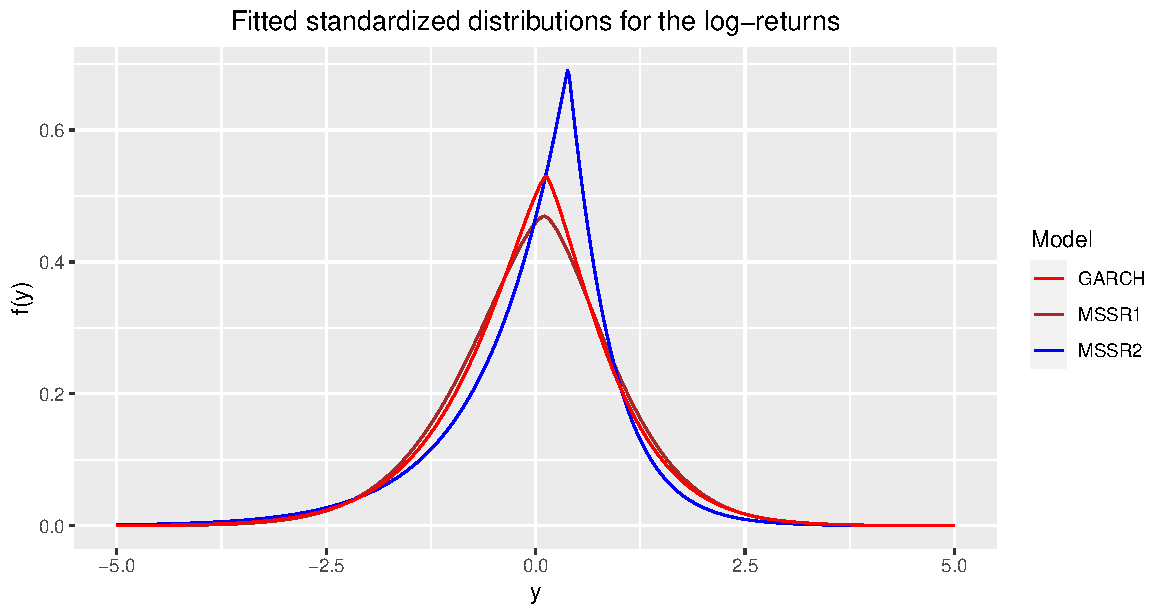
\includegraphics[width=0.7\linewidth]{FittedStandardizedDistr.pdf}
	\caption{Probability distribution functions}
	\end{subfigure} \\
	\begin{subfigure}{.5\textwidth}
		\centering
		\includegraphics[width=1\linewidth]{FittedStandardizedDistrLogLogRight.pdf}
		\caption{Log-log plot for the positive tails}
	\end{subfigure}
	\begin{subfigure}{.5\textwidth}
	\centering
	\includegraphics[width=1\linewidth]{FittedStandardizedDistrLogLogLeft.pdf}
	\caption{Log-log-plot for the negative tails} \label{fig:distributions-left-tail}
	\end{subfigure}
	\caption{}
	\label{fig:distributions}
\end{figure}

In \cref{fig:distributions} the probability density functions of each sate and their tail behaviours are displayed.
In the log-log-plots one observe see the heavier tails of MSSR2 compared to the other two densities, especially in the negative tail.

In \cref{img:single-state-forecasts} one can see the two states of the MSGARCH (MSSR1 and MSSR2) model produce different forecasts and how they compare to the stand-alone GARCH model. 
It can be observed that MSSR1 is less persistent, which is due to the smaller $\beta_1 = 0.7519$ compared to the larger $\beta_2 = 0.935$ of MSSR2.
Furthermore we see that MSSR1 has a higher base-level volatility and tends to forecast volatility spikes which are larger than those of MSSR2. This once again, is caused by the larger $\alpha$ values which characterise MSSR1.

\begin{figure}[H]
	\label{img:single-state-forecasts}
	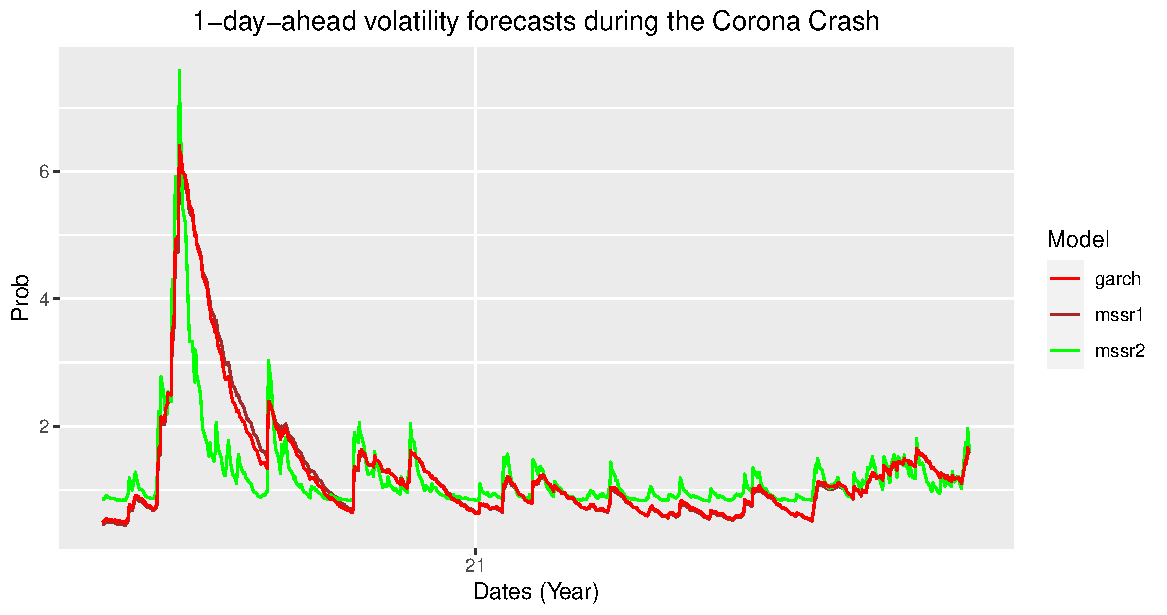
\includegraphics[width=\linewidth]{CoronaCrash_MSGARCH_Decomposition.pdf}
	\caption{One-day-ahead volatility forecasts during the Corona crash 2020. }
\end{figure}

%TODO insample performance evaluation ?

\subsubsection{Out-of-Sample Evaluation}
We evaluated the performance of our model in an out-of-sample dataset ranging from \formatdate{02}{10}{2003} to \formatdate{19}{08}{2022}. For every date the point and density forecasts are produced via simulation with a forecasting horizon ranging from 1 to 10 trading days. For this purpose 10000 future paths with length 10 are simulated at each step.

\begin{figure}[H]
	\label{fig:oos-error-multi-step}
	\begin{subfigure}{1.2\textwidth}
	\centering
	\includegraphics[width=\textwidth]{Forecast-Errors-OOS-Multi-Step.pdf}
	\end{subfigure}

	\begin{subfigure}{1.2\textwidth}
	\centering
	\includegraphics[width=\textwidth]{Forecast-Errors-OOS-Multi-Step2.pdf}
	\end{subfigure}
	\caption{Out-of-sample error measurements for different forecasting horizons and the two models MSGARCH and GARCH.}
\end{figure}


In \cref{fig:oos-error-multi-step} we can see that MSGARCH has slightly outperformed the GARCH model out-of-sample for every forecasting horizon from 1 to 10 days and for the three measures \ac{MSE}, \ac{MAE} and \ac{RMSE}. The density forecasts were even more similar in performance, here the GARCH model even  achieved slightly lower, i.e. better \ac{CRPS} values.

The percentage-wise improvement $\frac{e_{GARCH}-e_{MSGARCH}}{e_{GARCH}}$ (where e is the error measure) ranges from 2.14\% to 4\% for MSE and from 0.81\% to 3.2\% for MAE. It is not large, but consistent across error measures and forecasting horizons.
Both errors increase linearly with respect to the forecasting horizon, tending towards the error obtained by the unconditional volatility estimate.

%TODO: Error intervals


In \cref{fig:murphy-diagrams} the difference of the two forecasts in the murphy diagram are displayed. It can't be observed that any forecasting model dominates the other. This means that it depends on the error measure, whether the single-state GARCH or the MSGARCH forecasts produce smaller, more desireable errors.
Neither forecast is strictly better for all scoring rules which are consistent for the mean. For an explanation of murphy diagrams, see \cite{ehm_quantiles_2016} Sections 3 and 4.

\begin{figure}[H]
	\begin{subfigure}{.5\textwidth}
		\centering
		\includegraphics[width=.8\linewidth]{murph1.pdf}
		\caption{1a}
	\end{subfigure}%
	\begin{subfigure}{.5\textwidth}
		\centering
		\includegraphics[width=.8\linewidth]{murph2.pdf}
		\caption{1b}
	\end{subfigure}
	\begin{subfigure}{.5\textwidth}
	\centering
	\includegraphics[width=.8\linewidth]{murph3.pdf}
	\caption{1b}
\end{subfigure}
	\begin{subfigure}{.5\textwidth}
	\centering
	\includegraphics[width=.8\linewidth]{murph4.pdf}
	\caption{1b}
\end{subfigure}
	\caption{Plots showing the difference in the extremal scores of the MSGARCH and the GARCH forecasts for horizons 1-4.}
	\label{fig:murphy-diagrams}
\end{figure}


\subsection{Subsample Performance}
We further analyze the performance for two subsamples, which are categorized into a bull market and a bear market. For the bear market subsample we take the periods of 
\formatdate{22}{01}{2008} \textendash \formatdate{08}{07}{2009}, \formatdate{01}{02}{2020} \textendash \formatdate{13}{04}{2020} and \formatdate{01}{01}{2022} \textendash \formatdate{21}{08}{2022}.

\subsubsection{Bear Markets}
\begin{figure}[H]
	\label{fig:bear-error-multi-step}
	\begin{subfigure}{1.2\textwidth}
		\centering
		\includegraphics[width=\textwidth]{Forecast-Errors-BEAR-Multi-Step.pdf}
	\end{subfigure}
	
	\begin{subfigure}{1.2\textwidth}
		\centering
		\includegraphics[width=\textwidth]{Forecast-Errors-BEAR-Multi-Step2.pdf}
	\end{subfigure}
	\caption{Out-of-sample bear market subsample error measurements for different forecasting horizons and the two models MSGARCH and GARCH.}
\end{figure}

% TODO: Add scenario pictures

\subsubsection{Bull Markets}
\begin{figure}[H]
	\label{fig:bull-error-multi-step}
	\begin{subfigure}{1.2\textwidth}
		\centering
		\includegraphics[width=\textwidth]{Forecast-Errors-BULL-Multi-Step.pdf}
	\end{subfigure}
	
	\begin{subfigure}{1.2\textwidth}
		\centering
		\includegraphics[width=\textwidth]{Forecast-Errors-BULL-Multi-Step2.pdf}
	\end{subfigure}
	\caption{Out-of-sample bull market subsample error measurements for different forecasting horizons.}
\end{figure}

\section{Conclusion}
In this work the compared and analyzed the forecasting performance of a GARCH model with a \ac*{MSGARCH} for the S\&P using daily returns ranging from 1928 to 2022. We evaluated density forecasts as well as point forecasts for the volatility for different forecasting horizons. In this experiment we didn't see any significant evidence that would suggest that the markov-switching model produced superior forecasts compared to the single-regime \ac{GARCH} model. More experiments will have to be performed, including different model specifications, time horizons and indices in order to evaluate, if the markov-switching approach adds value in this setting.

\newpage


% Kopf- und Fußzeile definieren 
\pagestyle{fancy}						
\fancyhf{}								
%Kopfzeile rechts bzw. außen			
\fancyhead[R]{}							 
%Linie oben								 
\renewcommand{\headrulewidth}{0pt}	 
%Fußzeile mittig					 
\fancyfoot[R]{\thepage}				 
%Linie unten										
\renewcommand{\footrulewidth}{0pt}	 
%Seitenzahlen ab hier						 
\pagenumbering {Roman} 
\setcounter{page}{5}
\newpage\clearpage

\newpage
\bibliography{References}
\bibliographystyle{Alpha}


\begin{appendices}
%TODO add tables here
\chapter{Point Forecasts}
\label{app:point-forecasts}

\end{appendices}

\newpage

\begin{flushright}
$\overline{~~~~~~~~~~~~~~~\mbox{(Date, Signature)}~~~~~~~~~~~~~~~}$
\end{flushright}
\end{document}